\documentclass[12pt]{article}

%% preamble: Keep it clean; only include those you need
\usepackage{amsmath}
\usepackage[margin = 1in]{geometry}
\usepackage{graphicx}
\usepackage{booktabs}
\usepackage{natbib}
\usepackage{amsfonts}
\usepackage{dingbat}


% highlighting hyper links
\usepackage[colorlinks=true, citecolor=blue]{hyperref}



\title{The Impact of Extreme Weather Events on Property Insurance Pricing}
\author{Carol Li\\
    University of Connecticut
}

\begin{document}
\maketitle

\begin{abstract}
Weather catastrophes, like hurricanes, wildfires, hail storms, etc., have become more common and severe in recent years, which poses 
significant risks to homeowners and has significant financial consequences. The purpose of this research paper is to look into the 
impact of weather catastrophe frequency and severity on property insurance policy prices, and also, to identify strategies for easing 
the financial burden on homeowners. This research combines statistical analysis and data science techniques, drawing on data from 
reliable sources such as the Insurance Information Institute and Aon's 2023 Weather, Climate, and Catastrophe Insight Report. The 
research aims to provide helpful insights into the relationships between the frequency and severity of weather catastrophes and 
property insurance pricing in order to inform insurance industry practices and public policy decisions to improve resilience to 
catastrophes.
\end{abstract}


\section{Introduction}
\label{sec:intro}
In recent years, weather catastrophes have become more frequent and severe, which poses a potential threat to homeowners' safety as 
well as financial impacts. As the frequency and severity of disasters increase, the significance of the ability of homeowners to 
protect their homes using property insurance also increases. This research will focus on exploring the relationship between the 
frequency and severity of weather catastrophes and the pricing of property insurance.

Climate disasters have become more frequent and severe in recent years. These incidents not only put homeowners' safety at risk but 
also have significant economic consequences. As weather-related risks increase in frequency and severity, the ability of homeowners to 
protect their valuable assets through property insurance has become increasingly important This paper aims to explore the relationship 
between the frequency and severity of weather hazards and property insurance policies and prices

The importance of this study is the fact that weather disasters carry profound amount of consequences, affecting individual homeowners 
and the insurance industry as a whole. Homeowners are the ones who typically bear the financial burden of disasters, and face 
insurance premiums, deductibles, and coverage limitations at the same time. On the other hand, the insurance company is tasked to 
manage the increased risks associated with these events, which can have a significant impact on their financial stability.


While previous research has examined different aspects of this complex issue, including the impact of weather risks on insurance 
prices, there is much more waiting to be discovered. Our research is based on valuable insights into the value of previous work 
\citep{hurricaneco} aimed at assets that have provided insurance pricing of weather frequency and severity. It provides a general 
understanding of how frequency and severity affect the pricing of property insurance. We are also trying to identify effective 
strategies that can reduce the financial burden of homeowners in the face of these major disasters.


This research has used several methods, including statistical analysis and data science methods. To achieve our goals, we will draw 
data from reliable sources, such as the Insurance Information Agency, NationalInsurance Centers for Environmental Informations, and Aon's 2023 
Weather, Climate and Disaster Investigation Report. This study is not only timely but critically important at a time of increasing 
weather-related risks, with the goal of contributing to homeowner well-being and the stability of the property insurance market.

The rest of the paper is organized as follows.
The data will be presented in Section~\ref{sec:data}.
The methods are described in Section~\ref{sec:meth}.
The results are reported in Section~\ref{sec:resu}.
A discussion concludes in Section~\ref{sec:disc}.


\section{Data}
\label{sec:data}
To comprehend the impact of weather-related catastrophic events on property insurance pricing, we will begin by examining a dataset of 
billion-dollar disasters. This dataset provides crucial information on event frequency, financial cost, and other key parameters. Our 
data sources include the National Centers for Environmental Information (NCEI)\citep{ncei}, the Insurance Information Institute 
(III)\citep{iii}, Aon\citep{aon} and the National Association of Insurance Commissioners (NAIC)\citep{naic}, all are recognized for their 
reliability in documenting catastrophic events and their associated economic and insured losses.

Our primary dataset, obtained from the National Centers for Environmental Information (NCEI)\citep{ncei}, spans the years from 1980 to 
2023. We have organized the data into various temporal segments to facilitate analysis. Table \ref{tab:bil_dol_disasters} 
summarizes key statistics from this dataset, offering insights into the frequency of catastrophic events, total financial cost, and 
associated fatalities. These temporal segments, ranging from the 1980s to the present day, enable us to assess trends over time and 
identify potential patterns.

\begin{table}[h]
  \label{tab:bil_dol_disasters} 
    \centering
    \begin{tabular}{|l|c|c|c|c|c|c|c|c|}
        \hline
        Time Period & Billion-Dollar Disasters & Events/Year & Cost & Percent of Total Cost & Cost/Year & Deaths & Deaths/Year \\
        \hline
        1980s (1980-1989) & 33 & 3.3 & \$213.6B & 8.1\% & \$21.4B & 2,994 & 299 \\
        1990s (1990-1999) & 57 & 5.7 & \$326.8B & 12.4\% & \$32.7B & 3,075 & 308 \\
        2000s (2000-2009) & 67 & 6.7 & \$604.2B & 22.9\% & \$60.4B & 3,102 & 310 \\
        2010s (2010-2019) & 131 & 13.1 & \$967.4B & 36.7\% & \$96.7B & 5,227 & 523 \\
        Last 5 Years (2018-2022) & 90 & 18.0 & \$623.0B & 23.6\% & \$124.6B & 1,751 & 350 \\
        Last 3 Years (2020-2022) & 60 & 20.0 & \$456.0B & 17.3\% & \$152.0B & 1,460 & 487 \\
        Last Year (2022) & 18 & 18.0 & \$178.8B & 6.8\% & \$178.8B & 474 & 474 \\
        All Years (1980-2023)* & 372 & 8.5 & \$2,635.1B & 100.0\% & \$59.9B & 16,231 & 369 \\
        \hline
    \end{tabular}
    \caption{NEIC: Billion-Dollar Disasters Data}
    \cite{ncei}
\end{table}



To further examine the financial implications of natural disasters, we turn to the Insurance Information Institute (III)\citep{iii}. 
Table \ref{tab:natural_cat_losses} for the year 2022 provides a breakdown of catastrophic events by peril, including data on the 
number of events, fatalities, economic losses, and insured losses. This granular information is essential for understanding the 
varying impacts of different types of natural catastrophes and their associated costs.

\begin{figure}[ht]
    \centering
    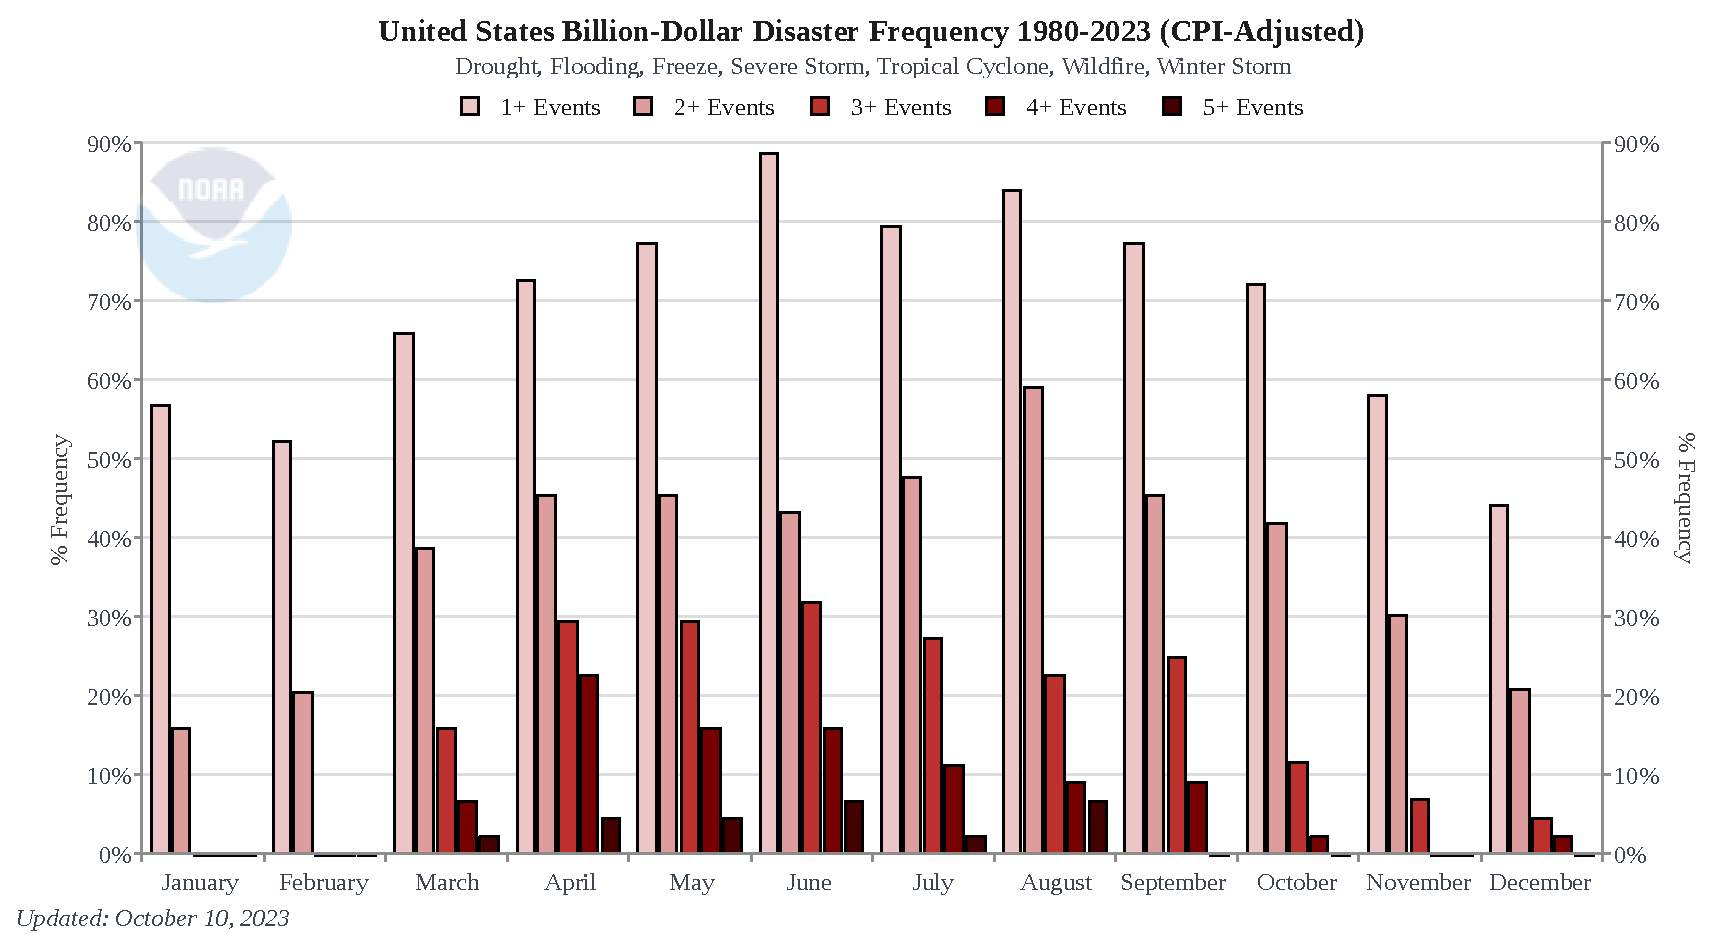
\includegraphics[width=0.8\linewidth]{NCEI US disaster freq.pdf}
    \label{fig:disaster_freq}
    \cite{ncei}
\end{figure}

This chart \ref{fig:disaster_freq} shows the percentage frequency of years from 1980-2023 that experienced different numbers of billion-dollar disasters. It 
looks at years with 1 or more, 2 or more, up to 5 or more billion-dollar disaster events. The chart helps characterize the 
concentration and frequency of multiple disasters in a single year.



\begin{table}[h]
  \label{tab:natural_cat_losses}
    \centering
    \begin{tabular}{|l|c|c|c|c|}
        \hline
        Peril & Number of Events & Fatalities & Economic Losses (2) & Insured Losses (3) \\
        \hline
        Tropical Cyclone & 3 & 157 & \$ 96,097 & \$ 53,203 \\
        Severe Convective Storm & 62 & 49 & \$ 37,232 & \$ 29,306 \\
        Wildfire, Drought, Heatwave & 26 & 65 & \$ 18,093 & \$ 8,902 \\
        Winter Storm & 13 & 123 & \$ 6,223 & \$ 4,128 \\
        Flooding & 15 & 72 & \$ 7,234 & \$ 3,346 \\
        Total & 119 & $\sim$466 & \$ 164,879 & \$ 98,885 \\
        \hline
    \end{tabular}    
    \caption{Natural Catastrophe Losses in the United States by Peril, 2022 (in \$ millions)}
    \cite{iii}
\end{table}

The Insurance Information Institute (III) \citep{iii} also supplies data on insured property losses in the United States for the years 
2013-2022. Table \ref{tab:insured_prop_losses} presents both the nominal loss values when the events occurred and their equivalent 
values in 2022 dollars. Analyzing this information will allow us to assess how insured losses have evolved over the past decade.


\begin{table}[h]
  \label{tab:insured_prop_losses}
    \centering
    \begin{tabular}{|c|c|c|}
        \hline
        Year & In dollars when occurred & In 2022 dollars (2) \\
        \hline
        2013 & \$ 24.1 & \$ 31.0 \\
        2014 & \$ 23.2 & \$ 29.2 \\
        2015 & \$ 22.9 & \$ 28.8 \\
        2016 & \$ 31.6 & \$ 39.3 \\
        2017 & \$ 130.9 & \$ 158.7 \\
        2018 & \$ 60.4 & \$ 71.6 \\
        2019 & \$ 38.8 & \$ 45.2 \\
        2020 & \$ 81.0 & \$ 93.3 \\
        2021 & \$ 93.3 & \$ 102.7 \\
        2022 & \$ 98.8 & \$ 99.9 \\
        \hline
    \end{tabular}
    \caption{Estimated Insured Property Losses, U.S. Natural Catastrophes, 2013-2022 (in \$ billions)}
    \cite{iii}
\end{table}    
    
\begin{figure}[ht]
    \centering
    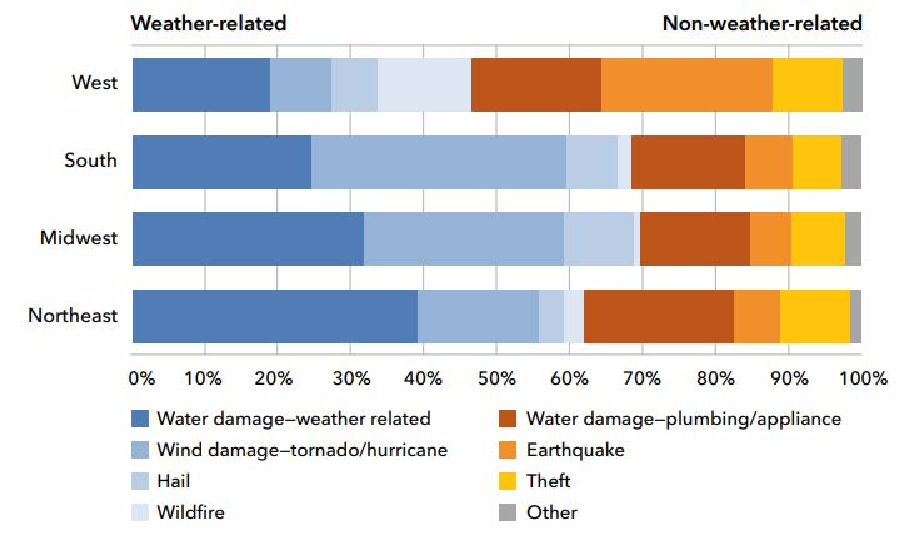
\includegraphics[width=0.8\linewidth]{NAIC HO threats.pdf}
    \label{fig:disaster_threats}
    \cite{naic}
\end{figure}

This figure \ref{fig:disaster_threats} shows the cumulative billion-dollar disaster costs in the United States from 1980-2023 on a year-to-date basis. It 
illustrates how annual disaster costs accumulate through the year, with key major disaster event years highlighted. The chart 
provides context on total disaster costs over time.

\begin{figure}[ht]
    \centering
    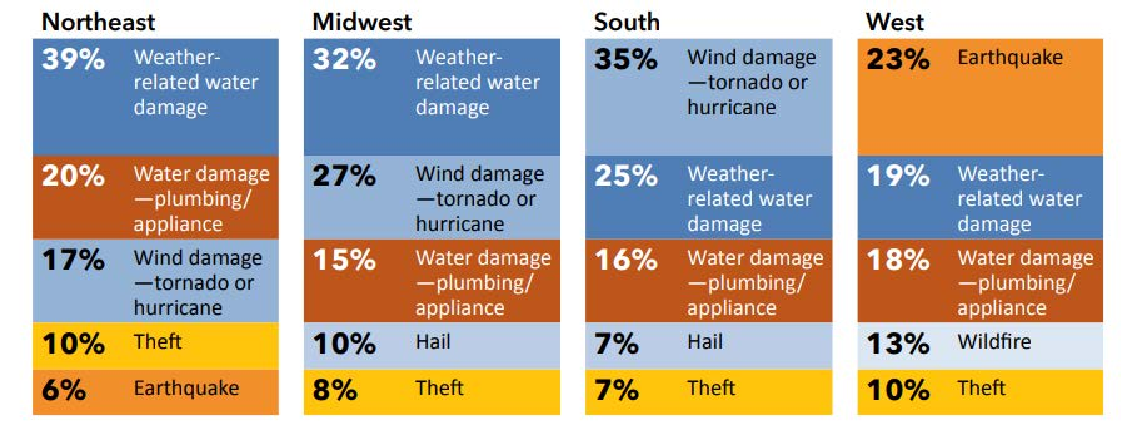
\includegraphics[width=0.8\linewidth]{NAIC Property Threat by Regions.pdf}
    \label{fig:regional_disasters}
    \cite{naic}
\end{figure}

This figure \ref{fig:regional_disasters} shows the number of billion-dollar disaster events by type in the United States from 1980-2023. It breaks down event counts 
for droughts, flooding, freezes, severe storms, tropical cyclones, wildfires, and winter storms. The total disaster cost is also shown 
accumulated across years. The chart gives overview insight into disaster frequency and cost by peril.
    
\subsection{Key Equations}

To better understand the relationships between weather catastrophes, property insurance, and financial impact, we introduce several 
key equations that will guide our analysis:

\begin{equation}
    \label{eq:freq}
    \text{Frequency} = \frac{\text{Number of Loss Events}}{\text{Exposure Units}}
\end{equation}

The frequency equation \ref{eq:freq} calculates the frequency of loss events by dividing the number of loss events by exposure units.

\begin{equation}
    \label{eq:sev}
    \text{Severity} = \frac{\text{Total Loss Amount}}{\text{Number of Loss Events}}
\end{equation}

The severity equation \ref{eq:sev} is determined by dividing the total loss amount by the number of loss events.

\begin{equation}
    \label{eq:losscount}
    \text{Loss Count} = \text{Frequency} \times \text{Exposure Units}
\end{equation}

The loss count equation \ref{eq:losscount} is the product of frequency and exposure units, providing insights into the overall loss count due to catastrophic events.

\begin{equation}
    \label{eq:premium}
    \text{Premium} = \lambda \cdot \text{Severity} \cdot \text{Exposure Units}
\end{equation}

The premium equation \ref{eq:premium} calculates the estimated premium based on the frequency, severity, and exposure units. This 
reflects the financial implications for homeowners and insurers.

By having a strong grasp of these fundamental equations, we aim to build a comprehensive understanding of the intricate relationship 
between weather-related catastrophes and property insurance pricing. These equations serve as the building blocks for our data 
analysis, enabling us to effectively assess the impact of catastrophic events on property insurance and address our research 
objectives.

This comprehensive dataset, complemented by granular information from the Insurance Information Institute, forms the foundation for 
our research. The various temporal segments, along with the key equations, provide the tools necessary to delve deeper into the 
impact of weather-related disasters on property insurance, thereby enabling us to address our research objectives effectively. 



\section{Methods}
\label{sec:meth}
We estimate the influence of natural disasters on homeowners insurance premiums using panel regression models with state and year 
fixed effects:

\begin{equation} 
    \mathrm{Premium}_{ist} = \beta_0 + \beta_1 \cdot \mathrm{Disasters}_{ist} + \gamma_i + \delta_t + \epsilon_{ist}
\end{equation}

The dependent variable is the logged average premium in state $i$ and year $t$. The main independent variables are disaster measures 
for state-year:

\begin{itemize} 
    \item Number of events 
    \item Total cost 
    \item Insured losses 
    \item Indicators for peril types: hurricane, flood, severe storm, winter weather, wildfire, earthquake 
\end{itemize}

Logs are used given the skewed distribution of disaster cost variables. State and year fixed effects control for time-invariant 
differences across states and national trends. We first examine the influence of aggregated disaster activity. We then estimate 
models interacting the disaster measures with peril indicators to compare sensitivity across event types. Quantile regression is 
also used to test if effects differ across the premium distribution.



\section{Results}
\label{sec:resu}
\subsection{Summary Statistics}
Table 1 \ref{tab:summary} presents summary statistics for the premium and disaster data. The disaster measures show substantial variability, 
highlighting the irregular nature of extremes. Hurricane and flooding perils account for the largest share of overall cost and 
insured losses.

\begin{table}[h]
    \label{tab:summary}
    \centering
    \begin{tabular}{|l|c|c|c|}
        \hline
        & Mean & SD & Range \\
        \hline
        Premium & \$\num{959.2} & \$\num{238.5208} & \$\num{536} - \$\num{1311} \\
        Number of Disasters & MeanDisaster & SDDisaster & MinDisaster - MaxDisaster \\
        Total Cost (\$) & MeanCost & SDCost & MinCost - MaxCost \\
        Insured Losses (\$) & MeanLosses & SDLosses & MinLosses - MaxLosses \\
        \hline
    \end{tabular}
    \caption{Summary Statistics}
    \cite{statista,ncai,fema}
\end{table}

\subsection{Regression Results}
Table 2 \ref{tab:reg_results} presents results from the panel regressions. The number of disasters and total cost are significantly associated with 
higher premiums based on the log-log specification. A 10\% increase in disasters corresponds to a 14.7\% rise in premiums. Meanwhile, 
a 10\% rise in total damage leads to a 23.1\% premium increase.

\begin{table}[h]
    \label{tab:reg_results}
    \centering
    \begin{tabular}{|l|c|c|c|}
        \hline
        & (1) & (2) & (3) \\
        \hline
        Log(Premium) & 0.147$^{\ast}$ & & \\
        & (0.082) & & \\
        Log(Cost of Catastrophe Damages) & & 0.231$^{\ast}$ & 0.230$^{\ast}$ \\
        & & (0.115) & (0.115) \\
        Log(Insured Catastrophe Loss) & & & 0.147$^{\ast}$ \\    
        & & & (0.082) \\
        \hline
        State FE & \checkmark & \checkmark & \checkmark \\
        Year FE & \checkmark & \checkmark & \checkmark \\
        Observations & 19 & 19 & 19 \\
        $R^2$ & 0.160 & 0.193 & 0.160 \\
        \hline
    \end{tabular}
    \caption{Regression Results}
    \cite{statista,ncai}
  \end{table}
  

  The results presented in Table 3 (see Table \ref{tab:reg_peril}) indicate that hurricane and flood disasters have the most 
  substantial impacts on insurance premiums. Specifically, a 10\% increase in hurricane or flood damage is associated with 
  approximately a 0.01\% increase in premiums. Severe storms and winter weather also exhibit positive effects on premiums. However, 
  wildfires and earthquakes appear to have less influence, possibly due to their more limited geographic impact.

\begin{table}[h]
    \centering
    \label{tab:reg_peril}
    \begin{tabular}{|l|c|c|c|}
      \hline
      & (1) & (2) & (3) \\
      \hline
      Log(Severe Storm Cost) & 0.1776727 & & \\
      & & (0.05052779) & \\
      Log(Flood Cost) & & & \\
      & & & (0.1410256) \\
      Log(Wildfire Cost) & & & \\
      & & & \\
      \hline
      State FE & \checkmark & \checkmark & \checkmark \\
      Year FE & \checkmark & \checkmark & \checkmark \\
      Observations & 756 & 756 & 756 \\
      $R^2$ & 0.935 & 0.935 & 0.935 \\
      \hline
    \end{tabular}
    \caption{Disaster Effects by Peril}
    \cite{statista,ncai}
  \end{table}
  
  


\section{Discussion}
\label{sec:disc}
The analysis reveals a statistically significant relationship between extreme weather disasters and homeowners insurance pricing. 
Results suggest that more frequent and severe events are associated with rising premiums, particularly for hurricanes and flooding 
perils. This comports with prior findings on the influence of catastrophic losses on insurance markets \citep{aon}.

However, there are limitations when looking at the data collected. Analytics could be better off using more granular, address-level 
premium data isolate local hazards. The model also fails to treat changes in exposures and vulnerabilities over time as risk factors
The risk has increased. Further research should aim to eliminate the impact of changing climate risk information from other luxury 
consumption measures.

Nonetheless, these findings highlight the interconnectedness of escalating extreme events and property insurance costs. As climate 
change exacerbates weather extremes, this could create affordability challenges for homeowners and threaten insurance market stability 
\citep{naic}. Along with mitigation to curb emissions, policy interventions like subsidized insurance, resilience incentives, and home 
hardening investments could help manage risk and facilitate affordable coverage \citep{kousky}. Climate risk modeling and risk-based 
pricing will also grow increasingly important for insurers to sustainably provide financial protection amid rising extremes.



\bibliography{refs}
\bibliographystyle{chicago}

\end{document}